\chapter{Propriétés des triangles}

\section{Droites et segments remarquables}

\subsection{Médiatrices}

\begin{definition}
    La \emph{médiatrice} d'un segment est la droite qui passe par le milieu du segment et qui lui est perpendiculaire.
\end{definition}

\begin{center}
	\begin{tikzpicture}
		\draw (0,0) -- (5,0);

        \draw[red] (2.5,-3) -- (2.5,3);

        \draw (0,-0.25) --  (0,0.25);
        \draw (5,-0.25) --  (5,0.25);

        \draw (1.125,-0.25) -- (1.375,0.25);
        \draw (3.625,-0.25) -- (3.875,0.25);

        \draw (2.25,0) -- (2.25,0.25) -- (2.5,0.25);
    \end{tikzpicture}
\end{center}

\begin{propriete}
    Si un point est sur la médiatrice d'un segment alors il est \emph{équidistant} des extrémités de ce segment. Réciproquement, si un point est équidistant des extrémités d'un segment, alors ce point est sur la médiatrice de ce segment.
\end{propriete}

\begin{center}
	\begin{tikzpicture}
        \draw (0,0) node[anchor = east]{$A$} -- (5,0) node[anchor = west]{$B$};

        \draw[blue] (0,0) -- (2.5,2.5) -- (5,0);

        \draw[red] (2.5,-3) -- (2.5,3);

        \draw (0,-0.25) --  (0,0.25);
        \draw (5,-0.25) --  (5,0.25);

        \draw (1.125,-0.25) -- (1.375,0.25);
        \draw (3.625,-0.25) -- (3.875,0.25);

        \draw (2.25,0) -- (2.25,0.25) -- (2.5,0.25);

        \draw (2.25, 2.5) -- (2.75, 2.5) node[anchor = west]{$M$};
    \end{tikzpicture}
\end{center}

\begin{exemple}
    Dans l'image au-dessus, les deux segments bleus sont de même longueur.
\end{exemple}

\begin{propriete}
    Les médiatrices des côtés d'un triangle non aplati sont concourantes en un point qui est le centre du cercle circonscrit à ce triangle. Si un triangle est rectangle, alors son hypoténuse est un diamètre de son cercle circonscrit.
\end{propriete}

\begin{propriete}
    Si l'un des côtés d'un triangle est un diamètre de son cercle circonscrit, alors ce triangle est rectangle (le diamètre du cercle circonscrit est alors son hypoténuse).
\end{propriete}

\subsection{Bissectrices}

\begin{definition}
    La bissectrice d'un angle est la droite qui partage cet angle en deux angles égaux.
\end{definition}

\begin{center}
	\begin{tikzpicture}
		\draw[red] (0,0) -- (5,0);

        \draw (1,0) -- (4,0.75);
        \draw (1,0) -- (4,-0.75);
    \end{tikzpicture}
\end{center}

\begin{propriete}
    Si un point est sur la bissectrice d'un angle, alors il est à égale distance des côtés de l'angle et inversement.
\end{propriete}

\begin{propriete}
    Les trois bissectrices d'un triangle sont concourantes. Leur point de concours, étant équidistant des trois côtés du triangle, est le centre d'un cercle tangent aux trois côtés du triangle. Ce cercle est appelé cercle inscrit au triangle.
\end{propriete}


\section{Théorème de Pythagore et réciproque}

\subsection{Théorème de Pythagore}

\begin{propriete}[Théorème de Pythagore]\label{chap5:pythagore}
    Dans un triangle rectangle, le carré de la longueur de l'hypoténuse (le côté opposé à l'angle droit) est égal à la somme des carrés des longueurs des deux autres côtés.
\end{propriete}

\begin{proof}
    La démonstration du théorème de Pythagore est particulièrement connue. Elle commence traditionnellement avec la figure suivante.
    \begin{center}
        \begin{tikzpicture}
            \draw (0,0) node[anchor=north east]{$A$}
                -- (5,0) node[anchor=north west]{$C$}
                -- (5,3) node[anchor=south west]{$B$}
                -- cycle;
            \draw (5,0) -- (5,3) -- (8,3) -- (8,0) -- cycle;
            \draw (0,0) -- (5,0) -- (5,-5) -- (0,-5) -- cycle;
            \draw (0,0) -- (5,3) -- (2,8) -- (-3,5) -- cycle;

            %\draw[dashed] (0.6765,7.2059)

            \draw (4.75,0) -- (4.75,0.25) -- (5,0.25);
        \end{tikzpicture}
    \end{center}
\end{proof}

% https://www.jchr.be/science/pythagore.htm

\begin{center}
	\begin{tikzpicture}
		\draw (0,0) node[anchor=north]{$A$}
            -- (5,0) node[anchor=north]{$C$}
            -- (5,3) node[anchor=south]{$B$}
            -- cycle;

        \draw (4.75,0) -- (4.75,0.25) -- (5,0.25);
    \end{tikzpicture}
\end{center}

Formule de Pythagore:
\[
    AB^2 = AC^2 + CB^2
\]

\begin{exemple}
    Pour le triangle suivant, nous avons d'après le théorème de Pythagore:
    \begin{align*}
        AB^2 & = AC^2 + CB^2\\
        \implies AB & = \sqrt{AC^2 + CB^2}\\
        \implies AB & = \sqrt{2.5^2 + 1.5^2}\\
        \implies AB & = \sqrt{6.25 + 2.25}\\
        \implies AB & = \sqrt{8.5} \text{ cm}\\
        \implies AB & \approx 2.92 \text{ cm}\\
    \end{align*}

    Donc $AB = \sqrt{8.5} \text{ cm} \approx 2.92 \text{ cm}$. \hfill
    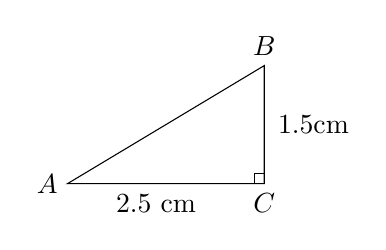
\begin{tikzpicture}
		\draw (0,0) node[anchor=east]{$A$}
            -- (2.5,0) node[anchor=north]{$C$}
            -- (2.5,1.5) node[anchor=south]{$B$}
            -- cycle;

        \draw (2.375,0) -- (2.375,0.125) -- (2.5,0.125);

        \draw (1.125,-0.25) node[anchor=center]{2.5 cm};
        \draw (3.125,0.75) node[anchor=center]{1.5cm};
    \end{tikzpicture}
\end{exemple}

\begin{exercice}
    Considérons le triangle $ABC$ rectangle en $B$. Nous savons que $AC = 5\text{ cm}$ et que $BA = 3 \text{ cm}$. Quelle est la longueur de $BC$?
\end{exercice}

\subsection{Réciproque du théorème de Pythagore}

Avant tout, que signifie le mot réciproque? Dans la Propriété~\ref{chap5:pythagore}, nous avons vu que si un triangle est rectangle, alors nous pouvons en déduire quelque chose. La réciproque inverse ces deux parties de la proposition: si nous avons que cette deuxième partie, alors nous pouvons en déduire la première partie. Attention, la réciproque d'une proposition n'est pas toujours vraie. Dans le cas du théorème de Pythagore cependant, elle l'est. Nous avons alors le résultat suivant:

\begin{propriete}\label{chap5:reciproque}
    Si dans un triangle, le carré du plus grand côté est égal à la somme des carrés des deux autres côtés, alors le triangle est rectangle (en le sommet opposé au plus grand côté).
\end{propriete}

\subsection{Contraposée du théorème de Pythagore}

\begin{propriete}
    Si dans un triangle, le carré du plus grand côté est différent de la somme des carrés des deux autres côtés, alors le triangle n'est pas rectangle.
\end{propriete}



\section{Théorème de Thalès}

Le théorème de Thalès est un autre théorème fondamental pour les relations entre distances au sein d'un triangle.